the time for which the graviton mass transitions from a nonzero value to zero.

There are multiple lines of evidence that point to the existence of a SGWB, and while many believe the background is mainly due to binary systems of supermassive black holes dispersed throughout the universe, more exotic cosmological sources cannot be excluded from consideration\cite{Agazie:2023}, including the possibility that the background is due to massive gravity;s amplification of primordial gravitational waves. 


The two models we will be considering have different functions for the mass and scale factor, as described in their respective papers \cite{Gumrukcuoglu:2012, Fujita:2018}. 

\begin{equation}\label{eqn:1}
    \mathcal{L}_h = \frac{a^2(\tau)M_{pl}}{8}[h_{ij}' h_{ij}' - \partial_lh_{ij}\partial_l h_{ij} - a^2(\tau)M_{GW}^2(\tau)h_{ij}h_{ij}]
\end{equation}
where $\tau$ is the conformal time defined by $\tau \equiv \int \frac{N(t)}{a(t)}dt$ where $N(t)$ is the lapse function, the primes (') denote derivatives with respect to $\tau$, $M_{pl}$ is the reduced Planck mass, $a(\tau)$ is the scale factor, and $M_{GW}(\tau)$ is the effective mass of gravitational waves. We will assume this and the graviton mass $m_g$ are the same. Additionally, we are only considering the tensor perturbations, which means that 
h_{ij} = \frac{2}{aM_{pl}}\sum_{\lambda \in \{+, \times\}} \int \frac{d^3 k}{(2\pi)^3}e^{i{\bf k \cdot x}}e^\lambda_{ij}[\gamma_k^\lambda(\tau)\hat{a}_{\bf k}^\lambda + \mbox{h.c.}] where $M_{pl}$ is the reduced Planck mass defined by $M_{pl} = (8\pi G)^{-1/2}$, ${\bf k}$ is the comoving momentum, $e^\lambda_{ij}$ is the polarization tensor, $a_{\bf k} / a_{\bf k}^\dagger$ are the creation/annihilation operators of the graviton, and h.c. is the hermitian conjugate. 

%\begin{figure}[h]
%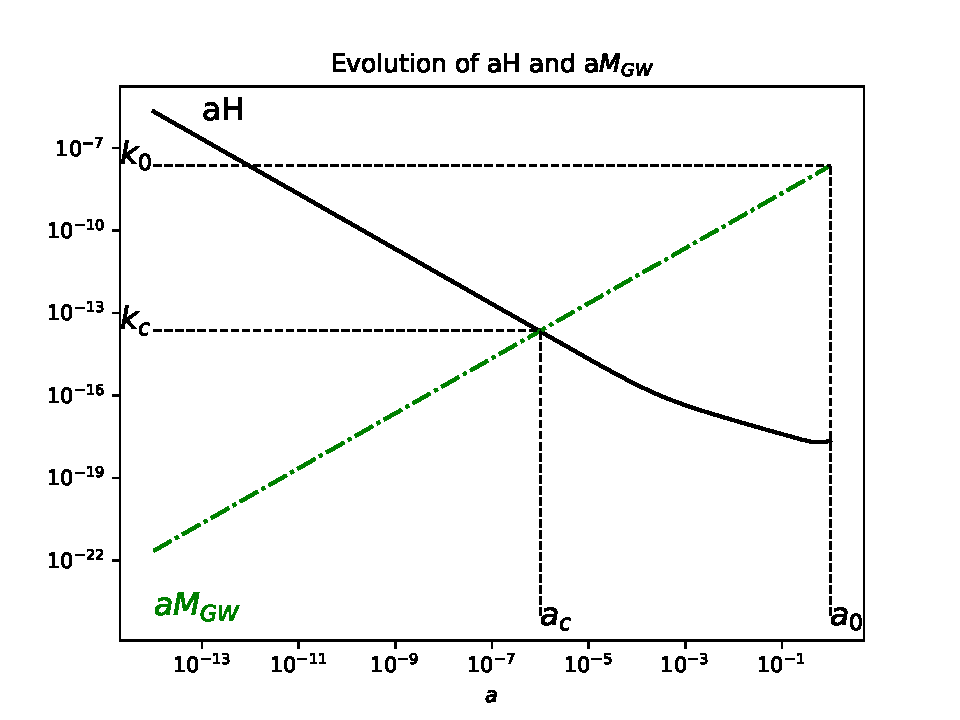
\includegraphics[scale=0.52]{fig/fig2.pdf}
%\caption{
%The evolution of $aH$ and $aM_{GW}$ as a function of $a$. Here, $M_GW$ is held constant. }
%\label{fig:kva}
%\end{figure}

= \left(\frac{a_{k'}^{GR} }{a_0}\right)^2 \left(\frac{k' a_k}{ka_{k'}^{GR}}\right)^2 \frac{\omega_k a_k}{\omega_0 a_0} P_{prim}(k) \\


\begin{figure*}
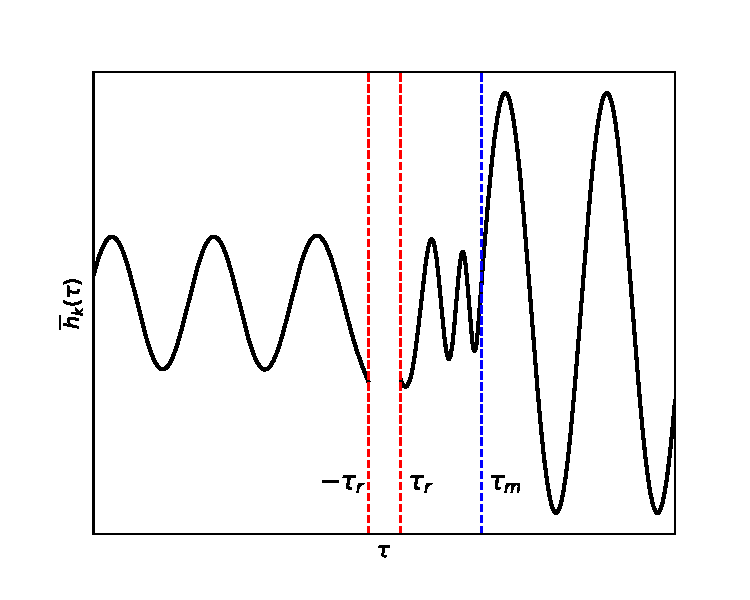
\includegraphics[width=\textwidth]{fig/fig1.pdf}
\caption{
GWB spectra produced by the CM model \cite{Gumrukcuoglu:2012}. We also show the $2\sigma$ and $4\sigma$ posterior median for the 15yr NANOGrav data set, in orange and in lighter orange respectively. The black dotted line is the GWB spectrum produced by an astrophysical population of inspiraling SMBHBs with the parameters detailed in Eq. A1 of \cite{Afzal:2023}. The red curve is the energy spectrum expected for a graviton with the same mass as the upper bound found in \cite{Wang:2023}, the blue curve is the energy spectrum for a graviton with the upper bound mass from \cite{Wu:2023}, and the green curve is the GWB spectra produced by a graviton with a mass determined by the lower frequency cutoff for NG15.}\label{fig:GWB_CM}
\end{figure*}

\begin{figure*}
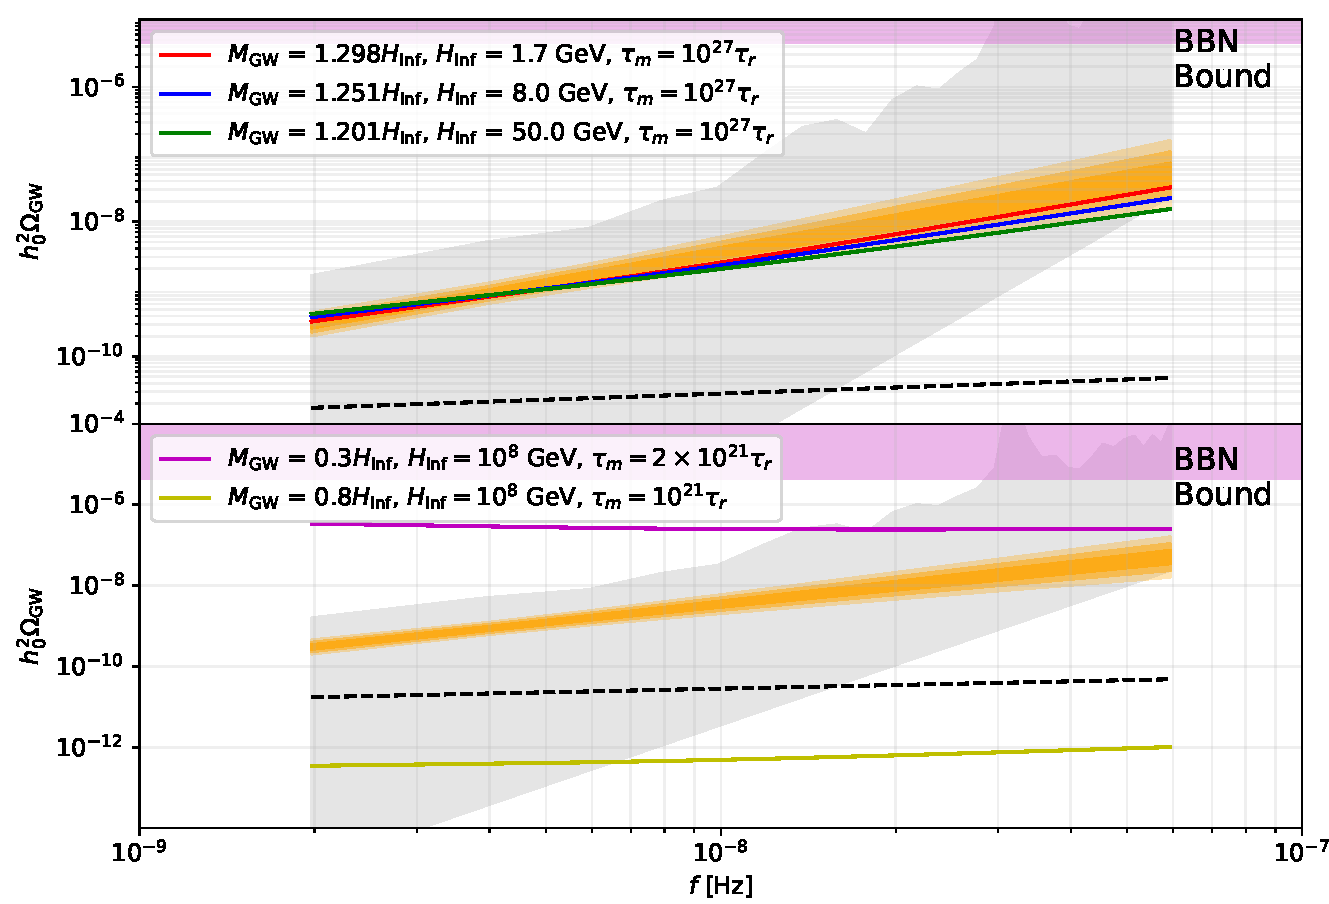
\includegraphics[width=\textwidth]{fig/fig3.pdf}
\caption{
GWB spectra produced by the SFM model \cite{Fujita:2018}. The orange contours and the black dotted line are the same as in Fig. \ref{fig:GWB_CM}. The blue curve is a GWB spectra from the SFM fitted to the $2\sigma$ posterior and the blue curve is fitted to the $4\sigma$ posterior. }\label{fig:GWB_SFM}
\end{figure*}


\subsection{Differences between the models}

\begin{figure}[h]
    \centering
    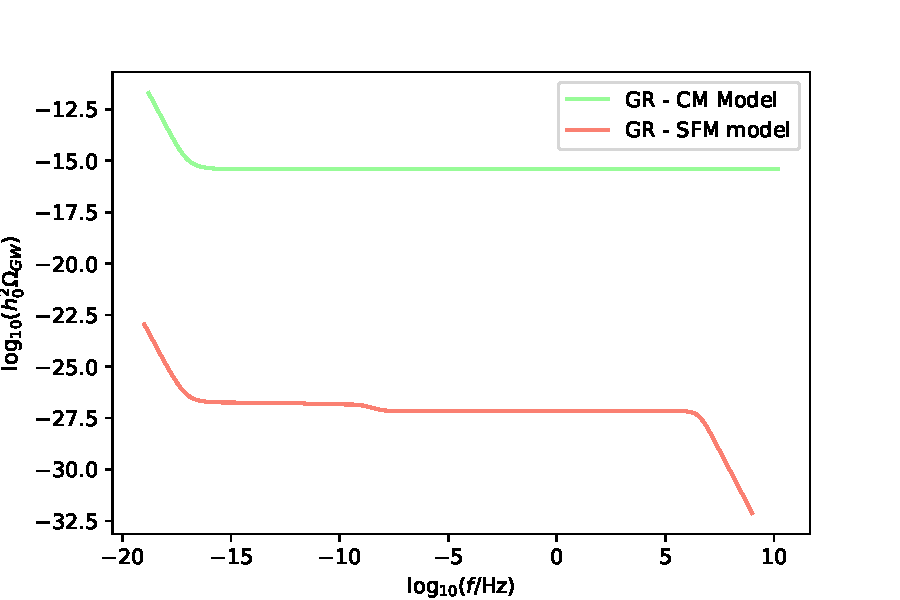
\includegraphics[width=\linewidth]{fig/fig5.pdf} 
    \caption{The massless GR energy spectra of the two models. The upper green one is the  }
\end{figure}
The two models use different GR primordial energy spectra. This discrepancy comes from the fact that in the CM model, the graviton mass is much less than the rate of Hubble expansion $H_{\inf}$ which leads to a scale-invariant primordial GW energy spectrum. In the SFM model, the mass is on the order of $H_{\inf}$, so the primordial GW energy density is blue-tilted \cite{Fujita:2018}, so we observe a  

The bound on $\Omega_{GW,0}$ made from the big bang nucleosynthesis (BBN) limits is cited in \cite{Fujita:2018}, which comes from the explicit limit on the integral of the energy density (Eq. 3.3 \cite{Tanin:2021}) 

\begin{equation} \label{eq:1}
    \int_{f = f_{BBN}}^{f = \infty}\mbox{d}(\ln{f}) h^2\Omega_{GW,0}(f) \lesssim 1\times 10^{-6}
\end{equation} 
where $f_{BBN}$ is the present day frequency of gravitational waves that were the same size as the horizon at the time of BBN, and the value is equal to $f_{BBN} \simeq 1.5\times 10^{-11} \ \Hz$. We can rewrite \eq{eq:1} as 
\begin{equation} \label{eq:11}
    \int_{f_{BBN}}^{\infty}\mbox{d}f \frac{1}{f} h^2\Omega_{GW,0}(f) \lesssim 1\times 10^{-6}
\end{equation} 


Thus, we see that the power spectrum takes on the form 
\begin{equation}\label{eqn:18}
    \begin{multlined}
    \mathcal{P}(\omega_0)  = \frac{\omega_0 a_k^3 \omega_k}{k^2 a_0} P_{prim}(k)\ .
    \end{multlined}
\end{equation}




\onecolumngrid
\begin{figure*}
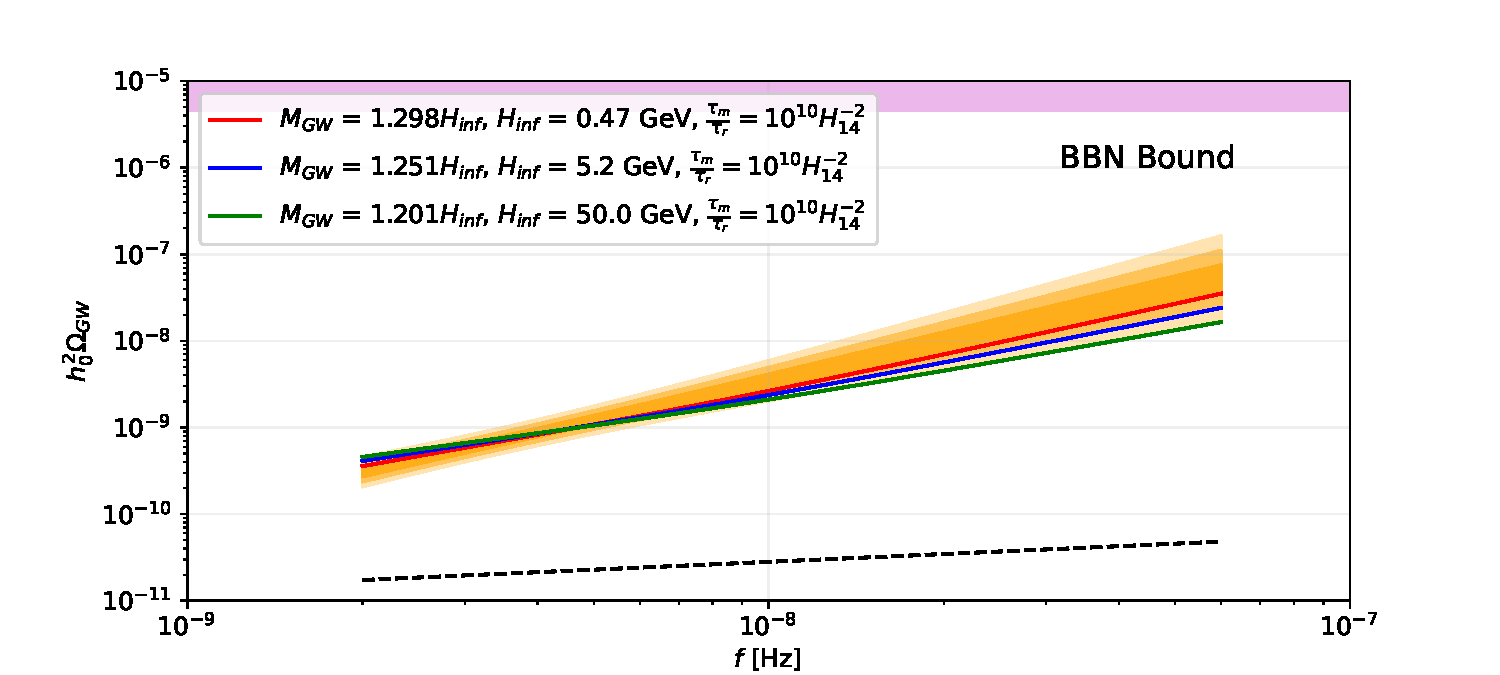
\includegraphics[width=\textwidth]{fig/fig8.pdf} 
\caption{GWB produced by the SFM model. We show the $1\sigma$, $2\sigma$, and $3\sigma$ posterior medians for NG15, in darker to lighter orange respectively. The black dotted line is the GWB spectrum produced by an astrophysical population of inspiraling supermassive black hole binaries with the parameters detailed in Eq.\ A1 of Ref.\ \cite{Afzal:2023}. The red curve is the GWB spectra fitted to the $1\sigma$ posterior, the blue curve is fitted to the $2\sigma$ posterior, and the green curve is fitted to the $3\sigma$ posterior. Here, $H_{14}$ is taken to be $H_{\inf} / 10^{14} \GeV$}
\label{fig:GWB}
\end{figure*}
\twocolumngrid


\begin{figure}[ht!]
\begin{subfigure}{.5\textwidth}
  \centering
  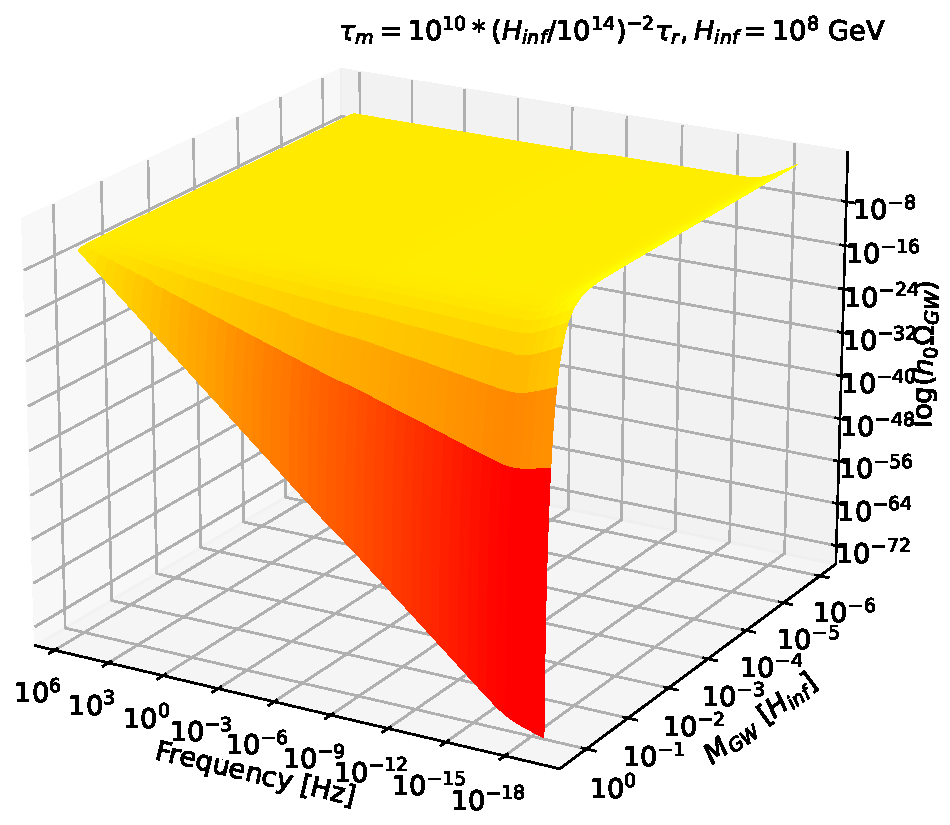
\includegraphics[width=.82\linewidth]{fig/fig4a.pdf}  
  \label{fig:contour-a}
\end{subfigure}
\begin{subfigure}{.5\textwidth}
  \centering
  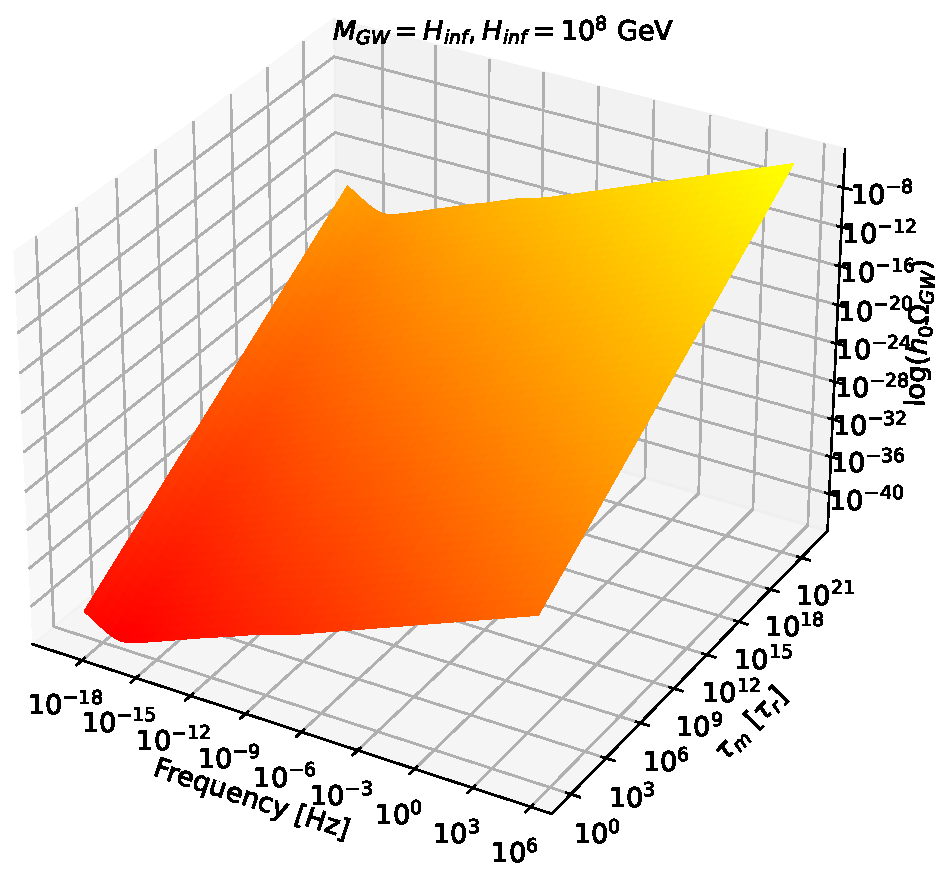
\includegraphics[width=.82\linewidth]{fig/fig4b.pdf}  
  \label{fig:contour-b}
\end{subfigure}
\begin{subfigure}{.5\textwidth}
  \centering
  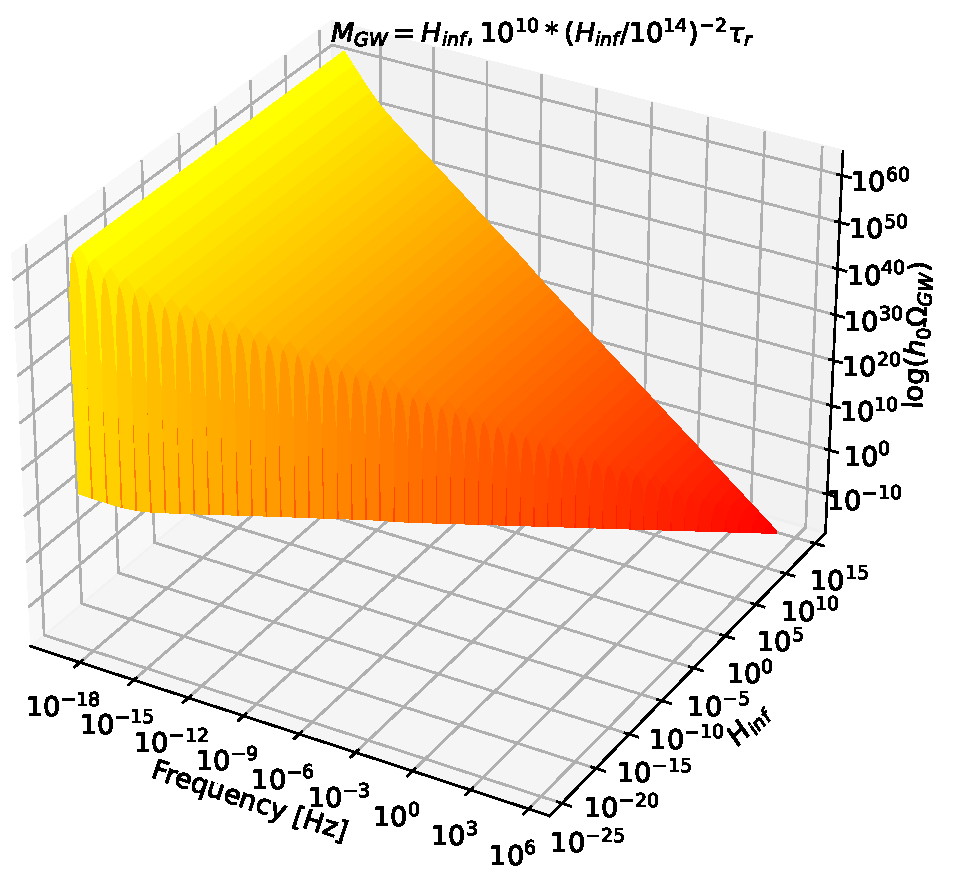
\includegraphics[width=.82\linewidth]{fig/fig4c.pdf}  
  \label{fig:contour-c}
\end{subfigure}
\caption{We plot $\Omega_{\text{GW},0}$ as a function of $f$ and $M$ (top), $\tau_m$ (middle), and $H_{\inf}$ (bottom). The frequency ranges from the scale corresponding to matter-radiation inequality ($\sim 3\times10^{-16}$ Hz) to the inflationary UV cutoff ($\sim 2\times 10^8\left(\frac{H_{\inf}}{10^{14} \GeV}\right)^{1/2}$ Hz \cite{Fujita:2018}).} 
\label{fig:contours}
\end{figure}


\begin{figure}[ht]
    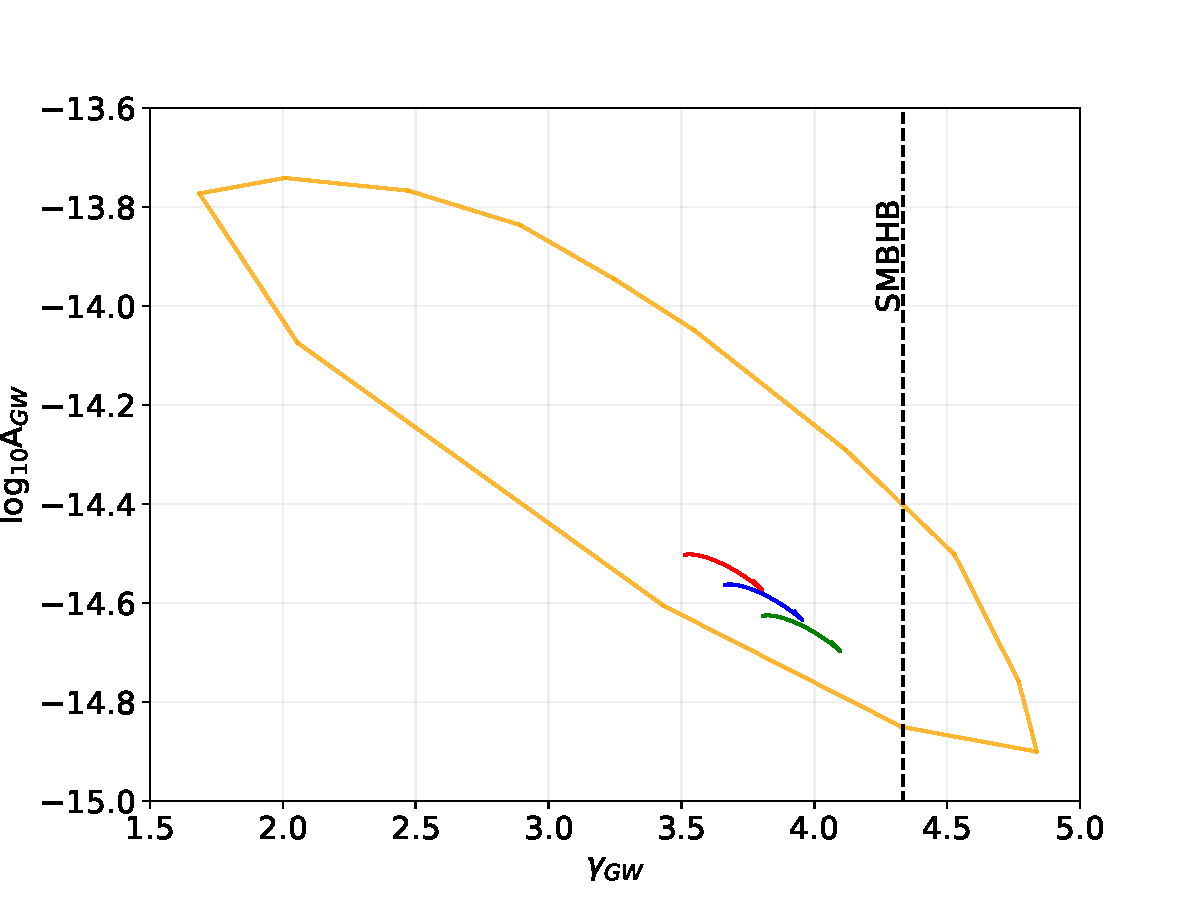
\includegraphics[width=\linewidth]{fig/fig9.pdf}
    \caption{Posterior probability distribution of the GWB amplitude and spectral index for the NANOGrav data. The value $\gamma_\text{GW}$ = 13/3 (dashed black line) represents the expected SMBHB spectrum. The amplitude is referenced to $f_{\text ref}$ = 1 yr$^{-1}$. The red, blue, and green curves represent the GWB spectra fitted to the $1\sigma$, $2\sigma$, and $3\sigma$ posterior of the signal.}
    \label{fig:amp_spec}
\end{figure}

\begin{figure}[ht!]
    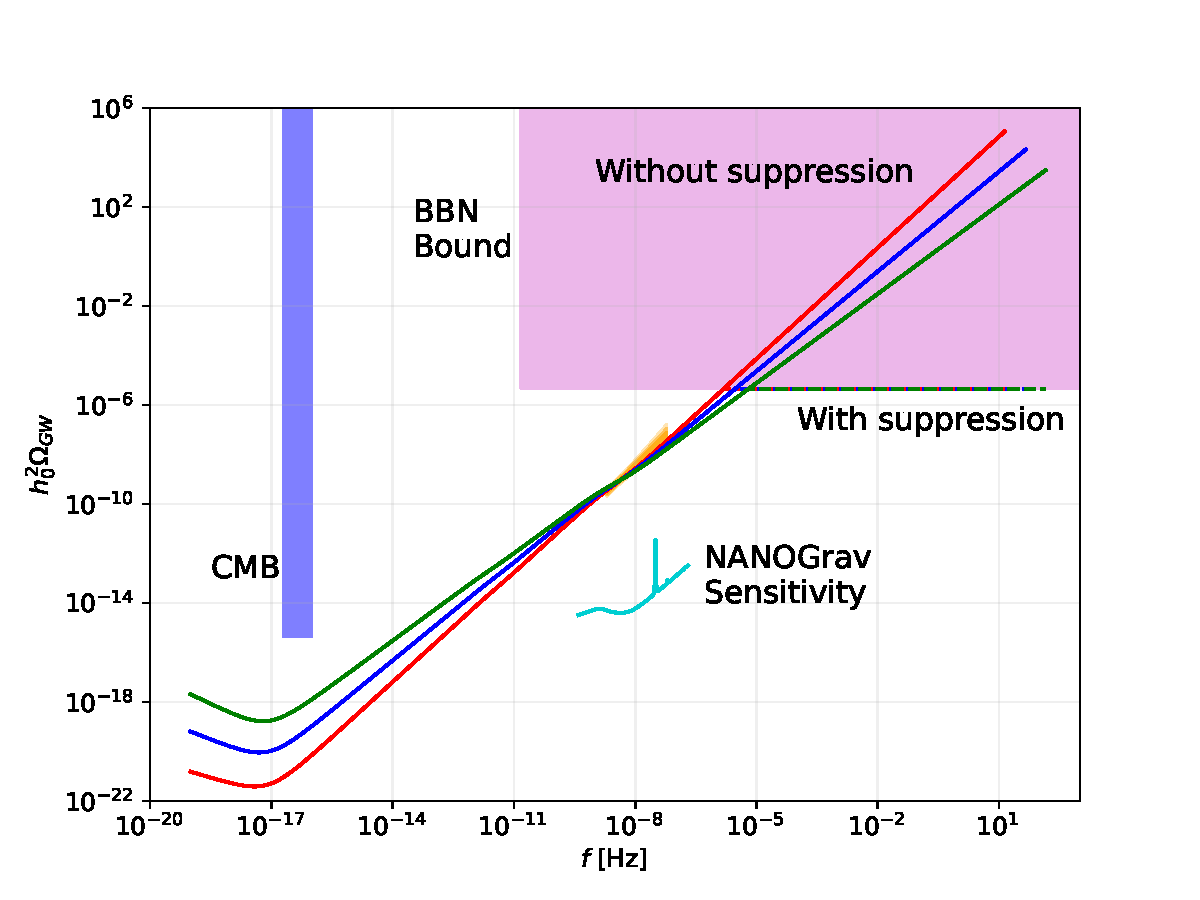
\includegraphics[width=\linewidth]{fig/fig7.pdf}
    \caption{The energy densities in Fig.\ \ref{fig:GWB} plotted over the whole frequency range specified in Fig.\ \ref{fig:contours}. The red, blue, and green curves correspond to the energy densities of the same color in Fig.\ \ref{fig:GWB}. The turquoise curve below the energy densities is the sensitivity curve for NANOGrav. The suppression takes place right before the energy density surpasses the BBN bound.}
    \label{fig:supp}
\end{figure}

We thank Prof.\ Shinji Mukohyama and Prof.\ Sachiko Kuroyanagi for insightful discussions on the nature of their models

%\begin{figure}[ht]
%    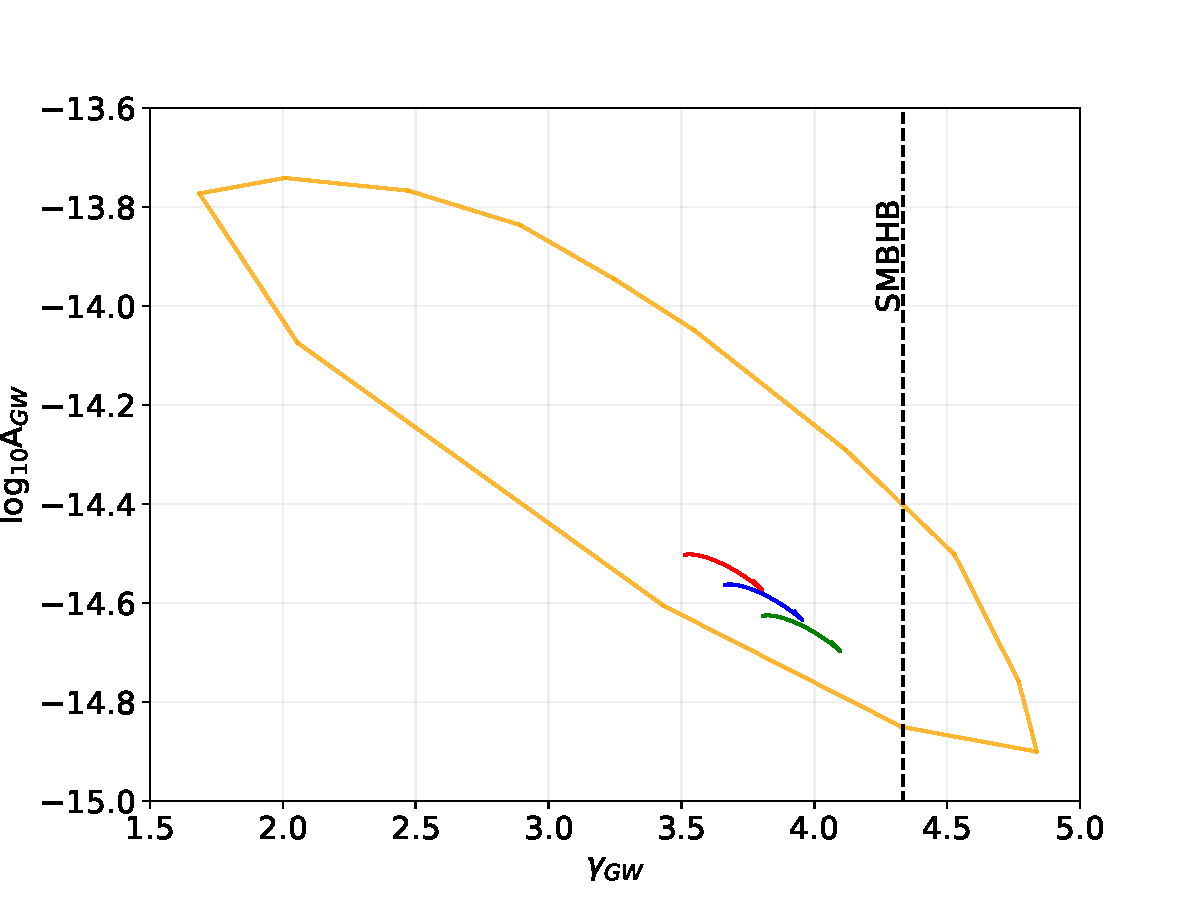
\includegraphics[width=\linewidth]{fig/fig9.pdf}
%    \caption{Posterior probability distribution of the GWB amplitude and spectral index for the NANOGrav data (orange). The value $\gamma_\text{GW}$ = 13/3 (dashed black line) represents the expected SMBHB spectrum. The amplitude is referenced to $f_{\text{ref}}$ = 1 yr$^{-1}$. The red, blue, and green curves represent the GWB spectra fitted to the $1\sigma$, $2\sigma$, and $3\sigma$ posterior of the signal.}
%    \label{fig:amp_spec}
%\end{figure}